%%%%%%%%%%%%%%%%%%%%%%%%%%%%%%%%%%%%%%%%%%%%%%%%%%%%%%%%%%%%%%%%%%%%%%%%%%%%%%%%%%%%%%%%%%%%%%%%%%%
%%%%%%%%%%%%%%%%%%%%%%%%%%%%%%%%%%%%%%%%%%%%%%%%%%%%%%%%%%%%%%%%%%%%%%%%%%%%%%%%%%%%%%%%%%%%%%%%%%%
%%%%%%%%%%%%%%%%%%%%%%%%%%%%%%%%%%%%%%%%%%%%%%%%%%%%%%%%%%%%%%%%%%%%%%%%%%%%%%%%%%%%%%%%%%%%%%%%%%%

\chapter{Metodología}

\section{Participantes}

Los sujetos fueron elegidos usando un muestreo \textit{no probabilístico por conveniencia} bajo los 
siguientes criterios de inclusión:
\begin{itemize}
\item Edad entre 60 y 85 años
\item Diestros (mano derecha dominante)
\item Sin ansiedad, depresión ni síndromes focales
\item No usar medicamentos o sustancias para dormir
\item Firma de consentimiento informado
\item Voluntario para el registro de PSG
\end{itemize}

Un total de 14 adultos mayores cumplieron los criterios de inclusión. Estos participantes fueron 
sometidos a una batería de pruebas neuropsicológicas para determinar su estado cognoscitivo general 
(Neuropsi, MMSE), descartar cuadros depresivos (GDS, SATS) y cambios en la vida cotidiana (KATZ).
%
En base a las pruebas se determinó que, objetivamente, 10 de los voluntarios no padecen depresión ni 
ansiedad, además de que no presentan afectaciones significativas en la vida diaria.

Para su análisis, los 10 participantes se dividieron en dos grupos en base a su estado cognoscitivo:
control (CTL) y con Probable Deterioro Cognitivo (PDC). 
%
Para esta clasificación se dio mayor atención al puntaje de Neuropsi, estandarizado según edad y 
escolaridad (cuadro \ref{puntajes}). 
%
El puntaje de MMSE se le otorgó menos importancia como clasificador debido a que tiene baja 
sensibilidad para el diagnóstico de deterioro cognitivo leve \cite{Ardila12}, y baja especificidad 
para individuos con escolaridad muy baja o muy alta \cite{Ostrosky00}.
%
Cabe mencionar que se entiende por especificidad a la probabilidad de un verdadero negativo, es 
decir que un individuo sin deterioro cognitivo obtenga un resultado de no-deterioro.

\begin{table}
\centering
\caption{Puntajes de corte para la prueba Neuropsi}
\begin{tabular}{llccrccc}
\toprule
&& \multicolumn{2}{l}{Sano} & \phantom{.} & \multicolumn{3}{l}{Deterioro cognitivo} \\
\cmidrule{3-4} \cmidrule{6-8} 
Escolaridad & Edad & Alto & Normal && Leve & Moderado & Severo\\
\midrule
Nula
& 16 -- 30 &\ppu 92 &\ppu 60 &&\ppu 45 & 30 & 14 \\
& 31 -- 50 &\ppu 95 &\ppu 68 &&\ppu 54 & 41 & 28 \\
& 51 -- 65 &\ppu 91 &\ppu 59 &&\ppu 44 & 28 & 13 \\
& 66 -- 85 &\ppu 76 &\ppu 48 &&\ppu 34 & 20 &\ppu 6 \\
\midrule
1 -- 4 años
& 16 -- 30 &    105 &\ppu 73 &&\ppu 58 & 42 & 27 \\
& 31 -- 50 &    105 &\ppu 81 &&\ppu 69 & 58 & 46 \\
& 51 -- 65 &\ppu 98 &\ppu 77 &&\ppu 67 & 57 & 47 \\
& 66 -- 85 &\ppu 90 &\ppu 61 &&\ppu 46 & 32 & 18 \\
\midrule
5 -- 9 años
& 16 -- 30 &    114 &    102 &&\ppu 97 & 86 & 75 \\
& 31 -- 50 &    118 &    106 &&    101 & 90 & 79 \\
& 51 -- 65 &    111 &\ppu 98 &&\ppu 91 & 79 & 67 \\
& 66 -- 85 &\ppu 97 &\ppu 80 &&\ppu 72 & 56 & 39 \\
\midrule
10 -- 24 años
& 16 -- 30 &    115 &    103 &&\ppu 98 & 87 & 77 \\
& 31 -- 50 &    113 &    102 &&\ppu 97 & 88 & 78 \\
& 51 -- 65 &    102 &\ppu 93 &&\ppu 88 & 80 & 72 \\
& 66 -- 85 &\ppu 92 &\ppu 78 &&\ppu 72 & 59 & 46 \\
\bottomrule
\multicolumn{5}{l}{Fuente: Ardila y Ostrosky \cite{Ardila12}}
\end{tabular}
\label{puntajes}
\end{table}

\begin{table}
\caption{Datos generales de los participantes}
\centering
\bordes{1.1}
{\small
\begin{tabular}{llcrrrrrrr}
\toprule
 \phantom{.}&
 & {Sexo} & {Edad} & {Escol.} & {Neuropsi} & {MMSE} & {SATS} & {KATZ} & {GDS} \\
\midrule
\multicolumn{6}{l}{\textbf{Grupo CTL}}\\
&VCR    & F    & 59\pz & 12\pz & 107\pz & 29\pz & 21\pz & 0\pz & 3\pz \\
&MJH    & F    & 72\pz & 9\pz  & 113\pz & 30\pz & 18\pz & 0\pz & 0\pz \\
&JAE    & F    & 78\pz & 5\pz  & 102\pz & 28\pz & 19\pz & 0\pz & 5\pz \\
&GHA    & M    & 65\pz & 9\pz  & 107.5  & 30\pz & 23\pz & 0\pz & 7\pz \\
&MFGR   & F    & 67\pz & 11\pz & 115\pz & 30\pz & 18\pz & 0\pz &      \\
\rowcolor{gris}
&\multicolumn{1}{c}{$\widehat{\mu}$} & 
               & 68.2  & 9.2   & 108.9  & 29.4  & 19.8  & 0.0  & 3.0  \\
\rowcolor{gris}
&\multicolumn{1}{c}{$\widehat{\sigma}$} & 
               & 7.2   & 2.7   & 5.2    & 0.9   & 2.2   & 0.0  & 3.0  \\
\midrulec
%\hline
\multicolumn{6}{l}{\textbf{Grupo PDC}}\\
&CLO    & F    & 68\pz & 5\pz  & 81\pz & 28\pz & 22\pz & 1\pz & 6\pz \\
&RLO    & F    & 63\pz & 9\pz  & 90\pz & 29\pz & 20\pz & 0\pz & 3\pz \\
&RRU    & M    & 69\pz & 9\pz  & 85\pz & 27\pz & 10\pz & 0\pz & 3\pz \\
&JGZ    & M    & 65\pz & 11\pz & 87\pz & 25\pz & 20\pz & 0\pz & 1\pz \\
&AEFP   & M    & 73\pz &  8\pz & 96\pz & 29\pz &   \pz & 0\pz & 2\pz \\
\rowcolor{gris}
&\multicolumn{1}{c}{$\widehat{\mu}$} & 
              & 67.6   & 8.4   & 87.8  & 27.4  & 18.0  & 0.2  & 3.0  \\
\rowcolor{gris}
&\multicolumn{1}{c}{$\widehat{\sigma}$} & 
              & 3.4    & 2.2   & 5.6   & 1.8   & 5.4   & 0.4  & 1.9  \\
\bottomrulec
\end{tabular} 
}
\label{tab_sujetos}
\end{table}

%%%%%%%%%%%%%%%%%%%%%%%%%%%%%%%%%%%%%%%%%%%%%%%%%%%%%%%%%%%%%%%%%%%%%%%%%%%%%%%%%%%%%%%%%%%%%%%%%%%
%%%%%%%%%%%%%%%%%%%%%%%%%%%%%%%%%%%%%%%%%%%%%%%%%%%%%%%%%%%%%%%%%%%%%%%%%%%%%%%%%%%%%%%%%%%%%%%%%%%

\section{Registro del polisomnograma}

Para llevar a cabo el registro, los adultos mayores participantes fueron invitados a acudir a las 
instalaciones del Laboratorio de Sueño, Emoción y Cognición, ubicado dentro del Instituto de Ciencias 
de la Salud (ICSa) dependiente de la Universidad Autónoma del Estado de Hidalgo. Los participantes 
recibieron instrucciones de realizar una rutina normal de actividades durante la semana que 
precedió al estudio, y se les recomendó no ingerir bebidas alcohólicas o energizantes (como café 
o refresco) durante las 24 horas previas al experimento, y que no durmieran siesta ese día.

Para efectuar el registro se usó un polisomnógrafo Medicid 5 (Neuronic Mexicana). El protocolo de 
PSG incluye: 
\begin{itemize}
\item 19 electrodos de EEG, colocadas siguiendo las coordenadas del Sistema Internacional 10--20
\item 2 electrodos de EOG para movimientos oculares horizontales y verticales
\item 2 electrodos de EMG colocados en los músculos submentonianos
\end{itemize}
%
Los electrodos para registro de EEG fueron montados usando los lóbulos auriculares como referencia
común; se mantuvo por debajo de \SI{50}{\micro\ohm}.

Las señales fueron amplificadas analógicamente usando amplificadores de alta ganancia en cadena, 
y adicionalmente fueron filtradas analógicamente usando filtros de paso de banda: 0.1--100 Hz 
para EEG, 3--20 Hz para EOG. 
Debido a dificultades técnicas el registro se efectuó a razón de 512 puntos por segundo (Hz) para 
algunos participantes, mientras que se usó 200 Hz para otros; en ambos casos se cumple la 
recomendación de la AASM de al menos 128 Hz.
%
Los registros digitalizados fueron almacenados en formato de texto bajo la codificación 
ASCII.

Los registros fueron segmentados en ventanas de 30 segundos de duración, referidas como 
\textit{épocas}, para su estudio posterior \textit{fuera de línea}. 
Usando los criterios de la AASM, cada una de las épocas fueron clasificadas según la etapa
de sueño como MOR o NMOR. Dicha clasificación fue llevada a cabo por expertos en sueño de ICSa.

\begin{table}
\centering
\caption{Datos generales sobre los registros de PSG}
\bordes{1.2}
{\small
\begin{tabular}{llcllcllr}
\toprule
    \phantom{.}&
    &\multirow{2}{*}{\bordes{1}\begin{tabular}{l}Frecuencia de\\ muestreo [\hz]\end{tabular}}
    \bordes{1.2}
    & \multicolumn{2}{c}{Total} & \phantom{l}   & \multicolumn{3}{c}{MOR*}\\
    \cmidrule{4-5}  \cmidrule{7-9}
    &&          &Puntos  &  Tiempo   &&Puntos  &  Tiempo   &  \% \\
\midrule
\multicolumn{6}{l}{\textbf{Grupo CTL}}\\
&VCR &200       &\ppu 5166000 & \ppu  7:10:30 &&\ppu 438000 &   0:36:30 & 8.48 \\
&MJH &512       &    15851520 & \ppu  8:36:00 &&    1950720 &   1:03:30 &12.31 \\
&JAE &512       &    13931520 & \ppu  7:33:30 &&    2626560 &   1:25:30 &18.85 \\
&GHA &200       &\ppu 6558000 & \ppu  9:06:30 &&\ppu 330000 &   0:27:30 & 5.03 \\
&MFGR&200       &\ppu 4932000 & \ppu  6:51:00 &&\ppu 570000 &   0:47:30 &11.56 \\

\rowcolor{gris}
&\multicolumn{1}{c}{$\widehat{\mu}$}  
              & &        & \ppu 7:51:30   &&        &   0:52:06 &11.25 \\
\rowcolor{gris}
&\multicolumn{1}{c}{$\widehat{\sigma}$} 
              & &        & \ppu 0:57:36   &&        &   0:23:00 & 5.13 \\
\midrulec

\multicolumn{6}{l}{\textbf{Grupo PDC}}\\
&CLO &512       &    14499840 & \ppu  7:52:00 &&    2027520 &   1:06:00 &13.98 \\
&RLO &512       &    12994560 & \ppu  7:03:00 &&    1520640 &   0:49:30 &11.70 \\
&RRU &200       &\ppu 2484000 & \ppu  3:27:00 &&\ppu 228000 &   0:19:00 & 9.18 \\
&JGZ &512       &    18539520 &      10:03:30 &&\ppu 506880 &   0:16:30 & 2.73 \\
&AEFP &512       &    14699520 &       7:58:30 &&\ppu 629760 &   0:20:30 & 4.28 \\

\rowcolor{gris}
&\multicolumn{1}{c}{$\widehat{\mu}$}  
              & &        & \ppu 7:16:48   &&        &   0:34:18 &8.38 \\
\rowcolor{gris}
&\multicolumn{1}{c}{$\widehat{\sigma}$} 
              & &        & \ppu 2:24:43   &&        &   0:22:14 &4.79 \\
\bottomrulec
\end{tabular}\\
*Dado que el sueño MOR aparece fragmentado, se reporta la suma de tales tiempos
}
\label{frecuencias}
\end{table}

%%%%%%%%%%%%%%%%%%%%%%%%%%%%%%%%%%%%%%%%%%%%%%%%%%%%%%%%%%%%%%%%%%%%%%%%%%%%%%%%%%%%%%%%%%%%%%%%%%%
%%%%%%%%%%%%%%%%%%%%%%%%%%%%%%%%%%%%%%%%%%%%%%%%%%%%%%%%%%%%%%%%%%%%%%%%%%%%%%%%%%%%%%%%%%%%%%%%%%%

\section{Aplicación de la prueba de Priestley-Subba Rao}

Se fragmentaron los registros en ventanas de 30 segundos de duración, sin traslape. Cada una de 
estas ventanas fue sometida a la prueba de PSR, y se clasificó como \textit{estacionaria en el 
sentido de PSR} si fue posible rechazar ($p<0.05$) la hipótesis de no-estacionariedad. 
%
Los resultados obtenidos (una lista de las épocas que son estacionarias) se guardaron en archivos 
de texto para su posterior análisis. 
%
Debido a la gran variabilidad entre el tiempo que los participantes pasaron en sueño MOR, se decidió
basar las comparaciones en proporciones de épocas; por ejemplo, se calculó la proporción de
épocas MOR que son estacionarias para todos los participantes.

\begin{figure}
\centering
\begin{lstlisting}[caption={}]
Priestley-Subba Rao stationarity Test for datos
-----------------------------------------------
Samples used              : 3072 
Samples available         : 3069 
Sampling interval         : 1 
SDF estimator             : Multitaper 
  Number of (sine) tapers : 5 
  Centered                : TRUE 
  Recentered              : FALSE 
Number of blocks          : 11 
Block size                : 279 
Number of blocks          : 11 
p-value for T             : 0.4130131 
p-value for I+R           : 0.1787949 
p-value for T+I+R         : 0.1801353 
\end{lstlisting}
\caption[Resultado típico para la función \texttt{stationarity}]
{Resultado típico para la función \texttt{stationarity}. La función de densidad espectral es
referida como SDF, mientras que los p valores. El p-valor para \texttt{T+I+R} corresponde al 
estadístico $S_{I+R}$, y el p-valor para \texttt{T} corresponde $S_T$
}
\label{res_psr}
\end{figure}

Como análisis exploratorio se graficaron en el tiempo las épocas, en todos los canales, como se 
muestra en la figura \ref{patroncito}. Este tipo de gráficos \textit{revelan} cierto tipo de 
\textit{bloques} de épocas estacionarias o no-estacionarias. Heurísticamente se puede afirmar que 
éstos patrones son independientes de la prueba de PSR, y anteriormente se reportó que estos patrones
suelen coincidir con la aparición de sueño MOR. Más adelante se ofrece una discusión al 
respecto.

\begin{figure}
\centering
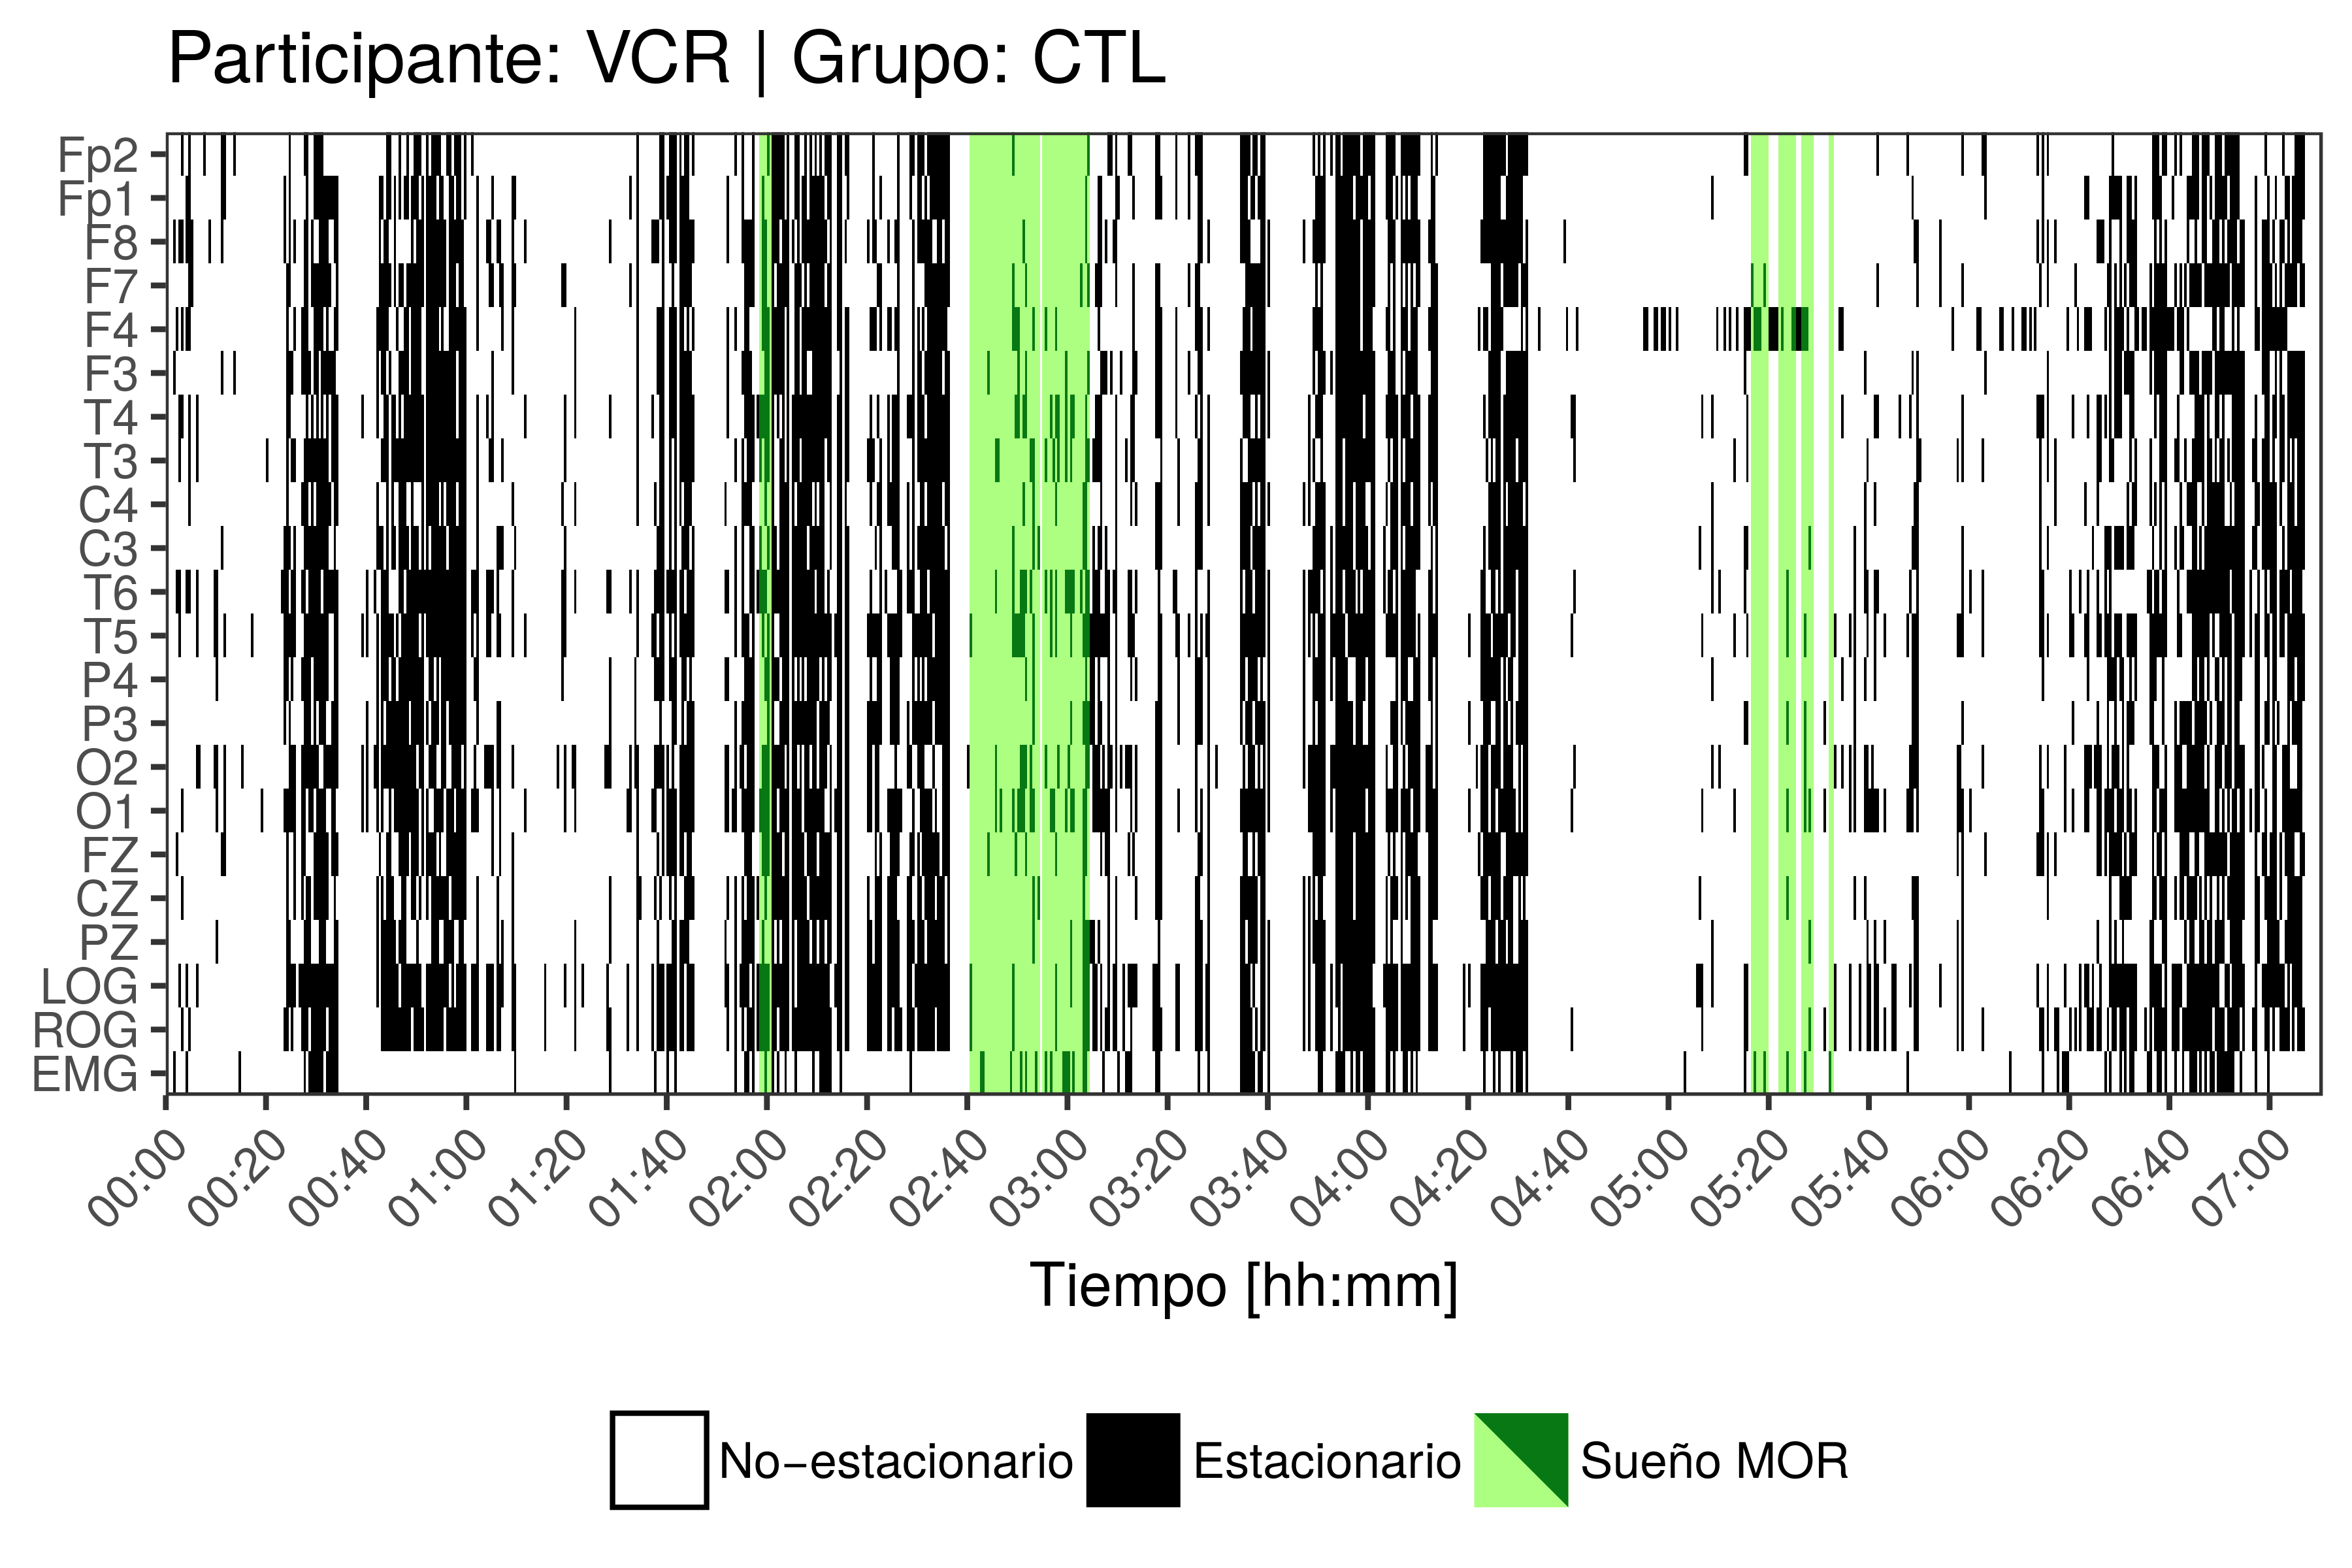
\includegraphics[width=.9\textwidth]
{./img_art_dfa/zoom_noVCR_v2.png} \\
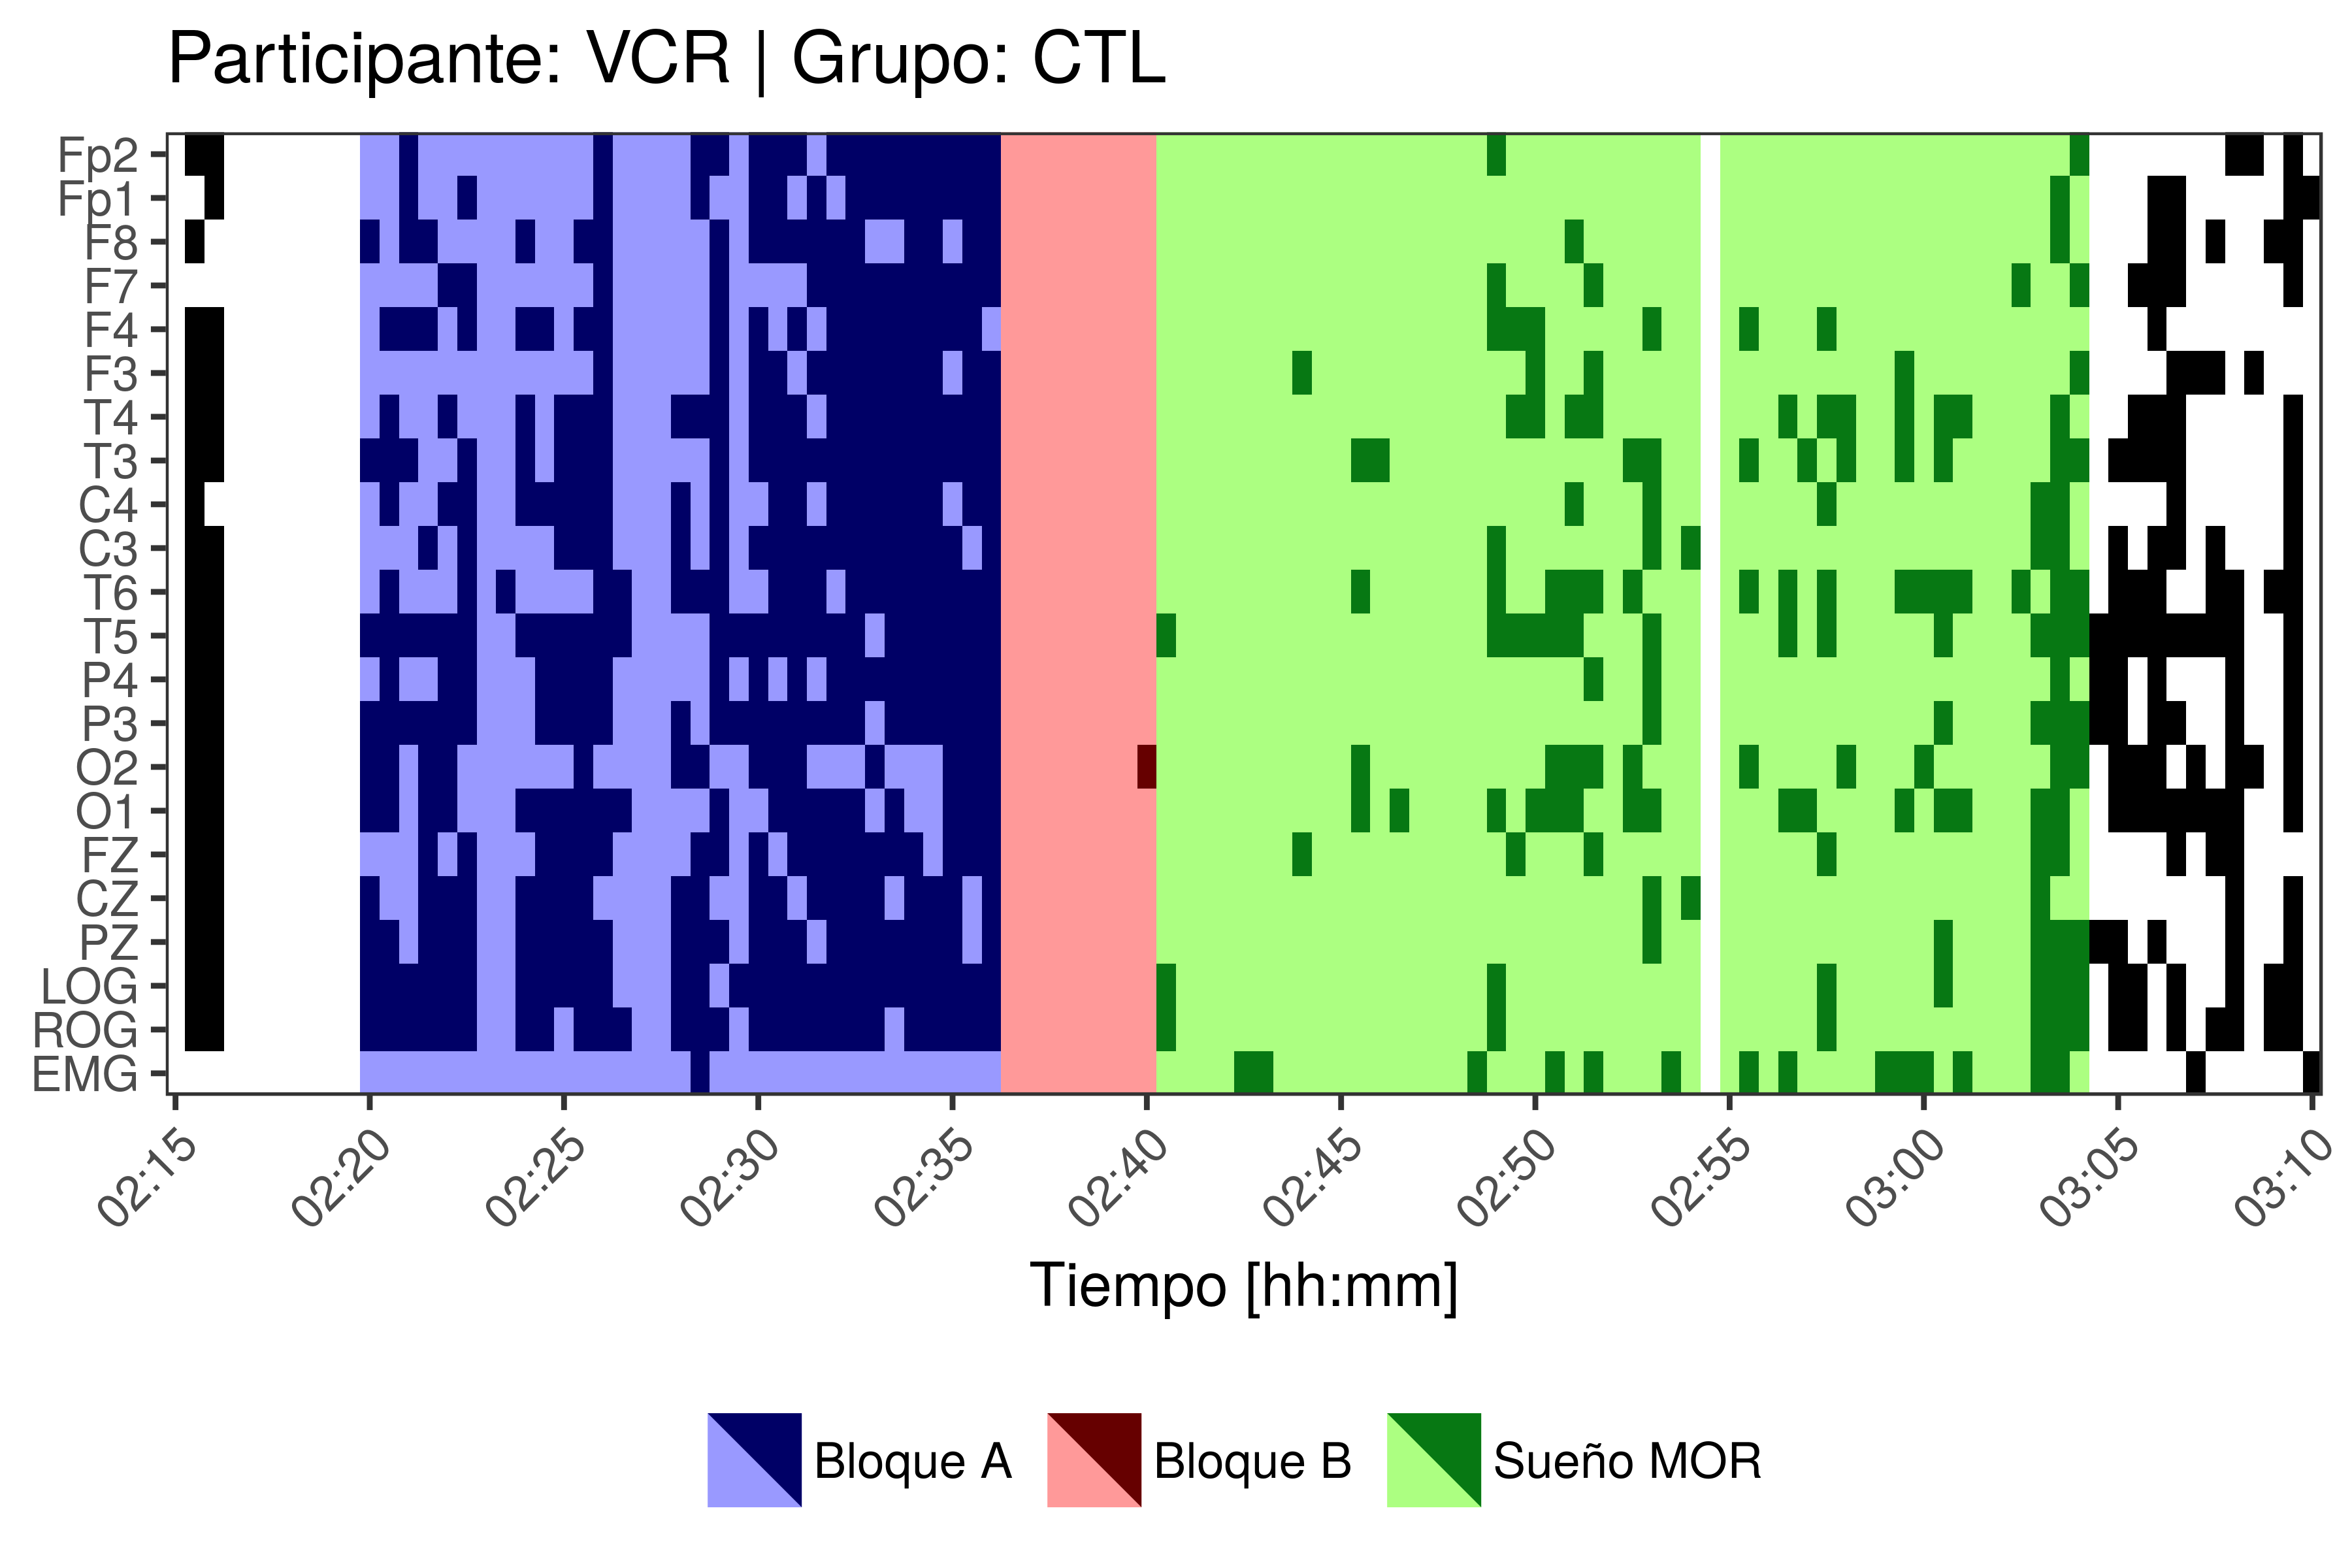
\includegraphics[width=.9\textwidth]
{./img_art_dfa/zoom_siVCR_v2.png}
\caption[Ubicación de épocas estacionarias en el tiempo y patrones emergentes]
{Ubicación de épocas estacionarias en el tiempo y patrones emergentes. \textbf{Arriba:} 
Ubicación de épocas estacionarias en el tiempo.
\textbf{Abajo:} Patrón de bloques relacionado con el sueño MOR}
\label{patroncito}
\end{figure}

En otro ámbito, se replicó la metodología usada por McEwen \cite{McEwen75} para contrastar la 
afirmación de que las series de tiempo \textit{suficiente cortas} son estacionarias. 
%
Este procedimiento consistió en repetir la clasificación de épocas variando el tamaño de ventana; 
los tamaños de ventana se tomaron de la forma $30 \times 2^{n}$ segundos, para comparar con el 
tamaño de época recomendado por la AASM.

Usando la clasificación de épocas estacionarias, obtenida para diferentes tamaños de ventana, se 
construyeron más gráficos sobre la ubicación de épocas estacionarias en el tiempo. Estos nuevos
gráficos, como el de la figura \ref{comp_VCR}, refuerzan heurísticamente la hipótesis de que los 
patrones son significativos fisiológicamente. 

En base a resultados previos usando esta técnica, se espera que el comportamiento de los patrones 
visuales obedezca al fenómeno de \textbf{estacionariedad local}; esta característica, descrita por 
Dahlhaus \cite{Dahlhaus97}, implica que un proceso puede ser aproximado a trozos 
\textit{ensamblando} procesos estacionarios.
%
Esta caracterización del EEG ha sido usada anteriormente de manera fructífera pero problemática
\cite{Barlow85,Kaplan99}.
%
Dentro del modelo para registros de PSG, la estacionariedad local significa que el PSG no es
formalmente homogéneo \textit{pero} puede entenderse como varios segmentos homógeneos. En un
sentido más general, es coherente pensar que el PSG se componga tanto de segmentos homógeneos
como de \textit{eventos puntuales} y artefactos.

En la figura \ref{epocas_diferentes} se muestra esquemáticamente cómo el tamaño
de las ventanas puede influir para su clasificación como estacionarias/homogéneas.

Entonces, se propone que los registros de PSG se comportan como procesos localmente estacionarios; 
más aún, se propone que esta característica cambia cualitativamente en adultos mayores con PDC,
para los cuales el \textit{nivel de homogeneidad} del PSG es muy similar durante MOR y NMOR.

\begin{figure}
\centering
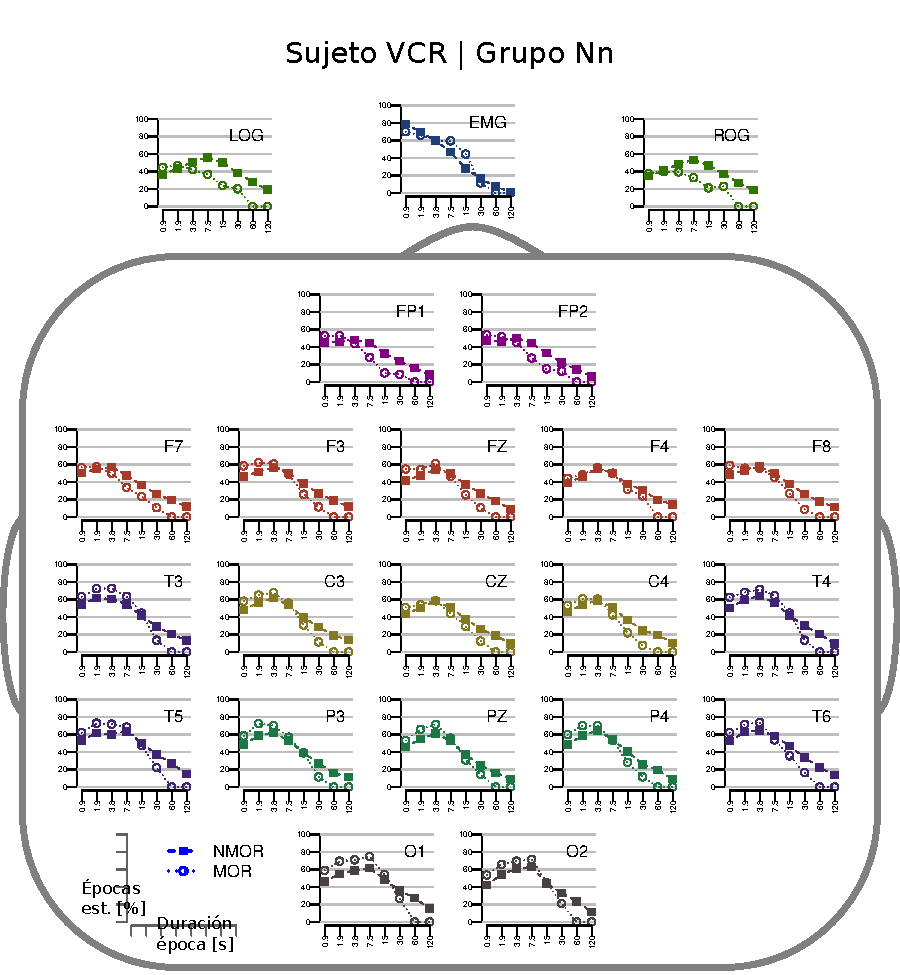
\includegraphics[width=.9\linewidth]{./img_resultados/cabeza_VCR.pdf}
\caption{Cambio en el porcentaje de épocas estacionarias conforme el tamaño de ventana}
\label{cabeza_repoio}
\end{figure}

\begin{figure}
\centering
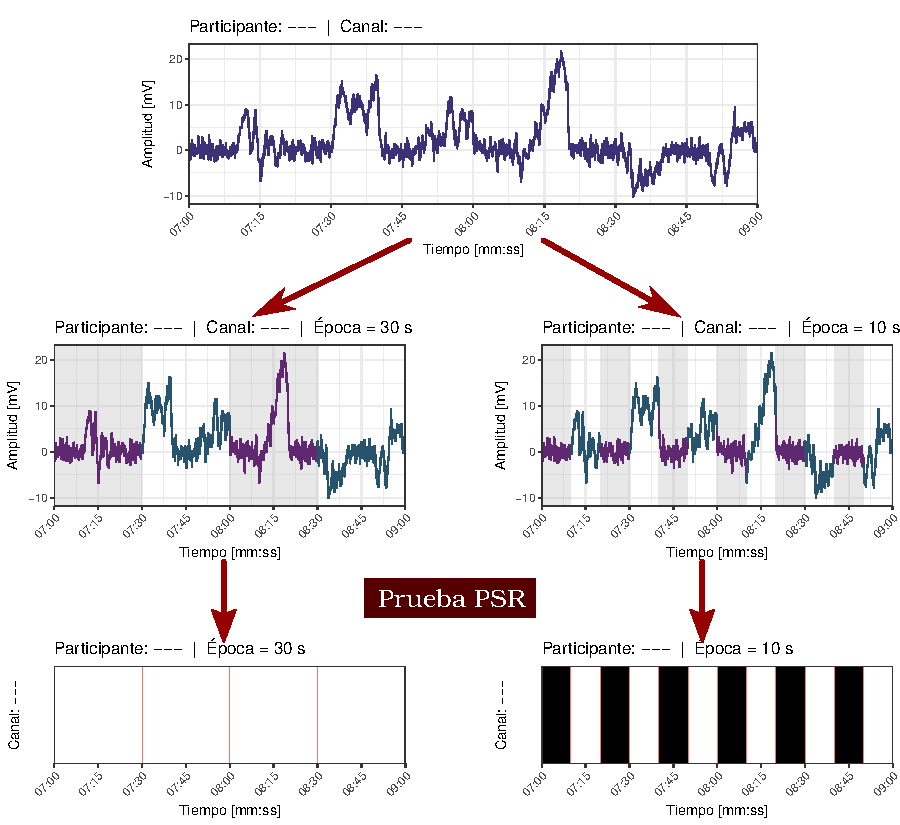
\includegraphics[width=\linewidth]{./img_diagramas/epocas_diferentes_v3.pdf}
\caption{Efecto del tamaño de ventana sobre la clasificación de estacionariedad.}
\label{epocas_diferentes}
\end{figure}

\begin{figure}
\centering
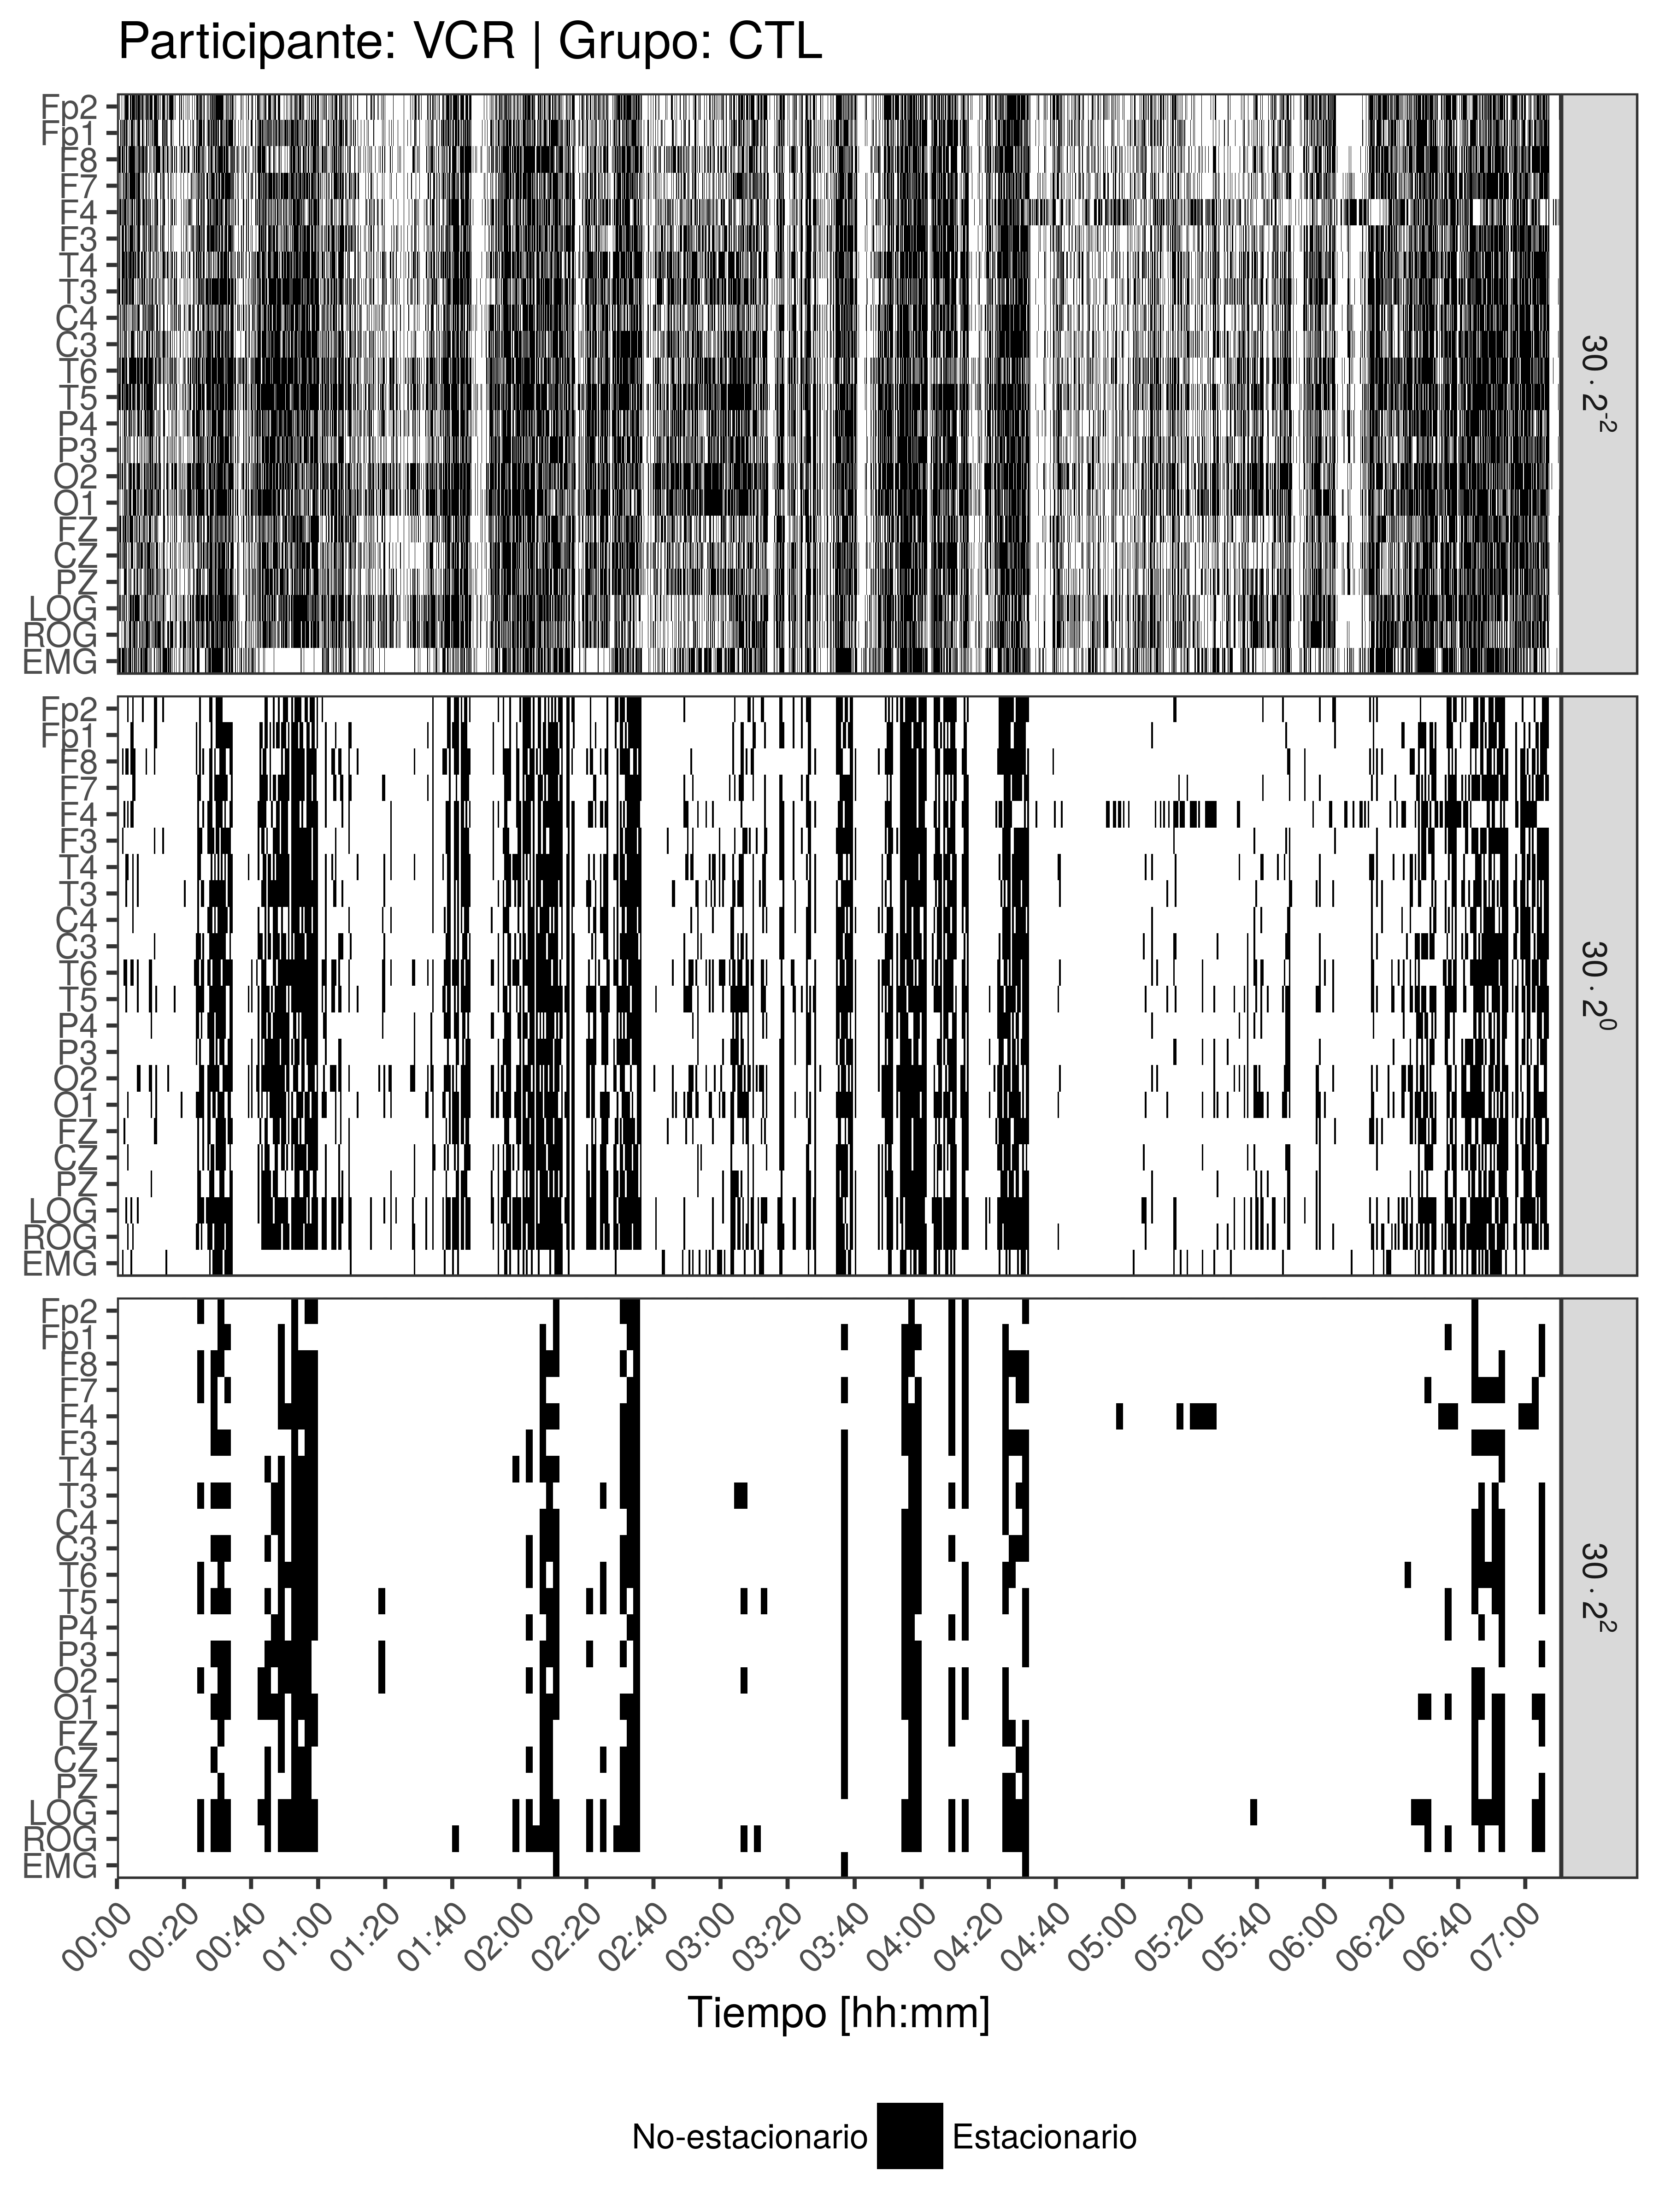
\includegraphics[width=\linewidth]
{./img_art_dfa/VCNNS1_comp_est_.png}
\caption{Distribución en el tiempo de ventanas estacionarias, usando diferentes tamaños
de ventana.}
\label{comp_VCR}
\end{figure}

Cabe destacar que la aplicación \textit{per se} de la prueba fue efectuada usando el software 
estadístico R \cite{R_citar}. En particular, se utilizó la implementación 
incluida en el paquete \texttt{fractal} \cite{R_fractal} bajo la función \texttt{stationarity}.

%%%%%%%%%%%%%%%%%%%%%%%%%%%%%%%%%%%%%%%%%%%%%%%%%%%%%%%%%%%%%%%%%%%%%%%%%%%%%%%%%%%%%%%%%%%%%%%%%%%
%%%%%%%%%%%%%%%%%%%%%%%%%%%%%%%%%%%%%%%%%%%%%%%%%%%%%%%%%%%%%%%%%%%%%%%%%%%%%%%%%%%%%%%%%%%%%%%%%%%

\section{Espectro de potencias}

Adicionalmente a la clasificación de épocas como estacionarias, se calculó su espectro de potencia. 
Como una metodología común, se calculó el \textbf{espectro de banda ancha},
es decir, la potencia total y relativa correspondientes a las frecuencias que caracterizan las ondas 
delta, theta, alfa, beta y gamma (ver cuadro \ref{tabla_ondas}).

\begin{figure}
\centering
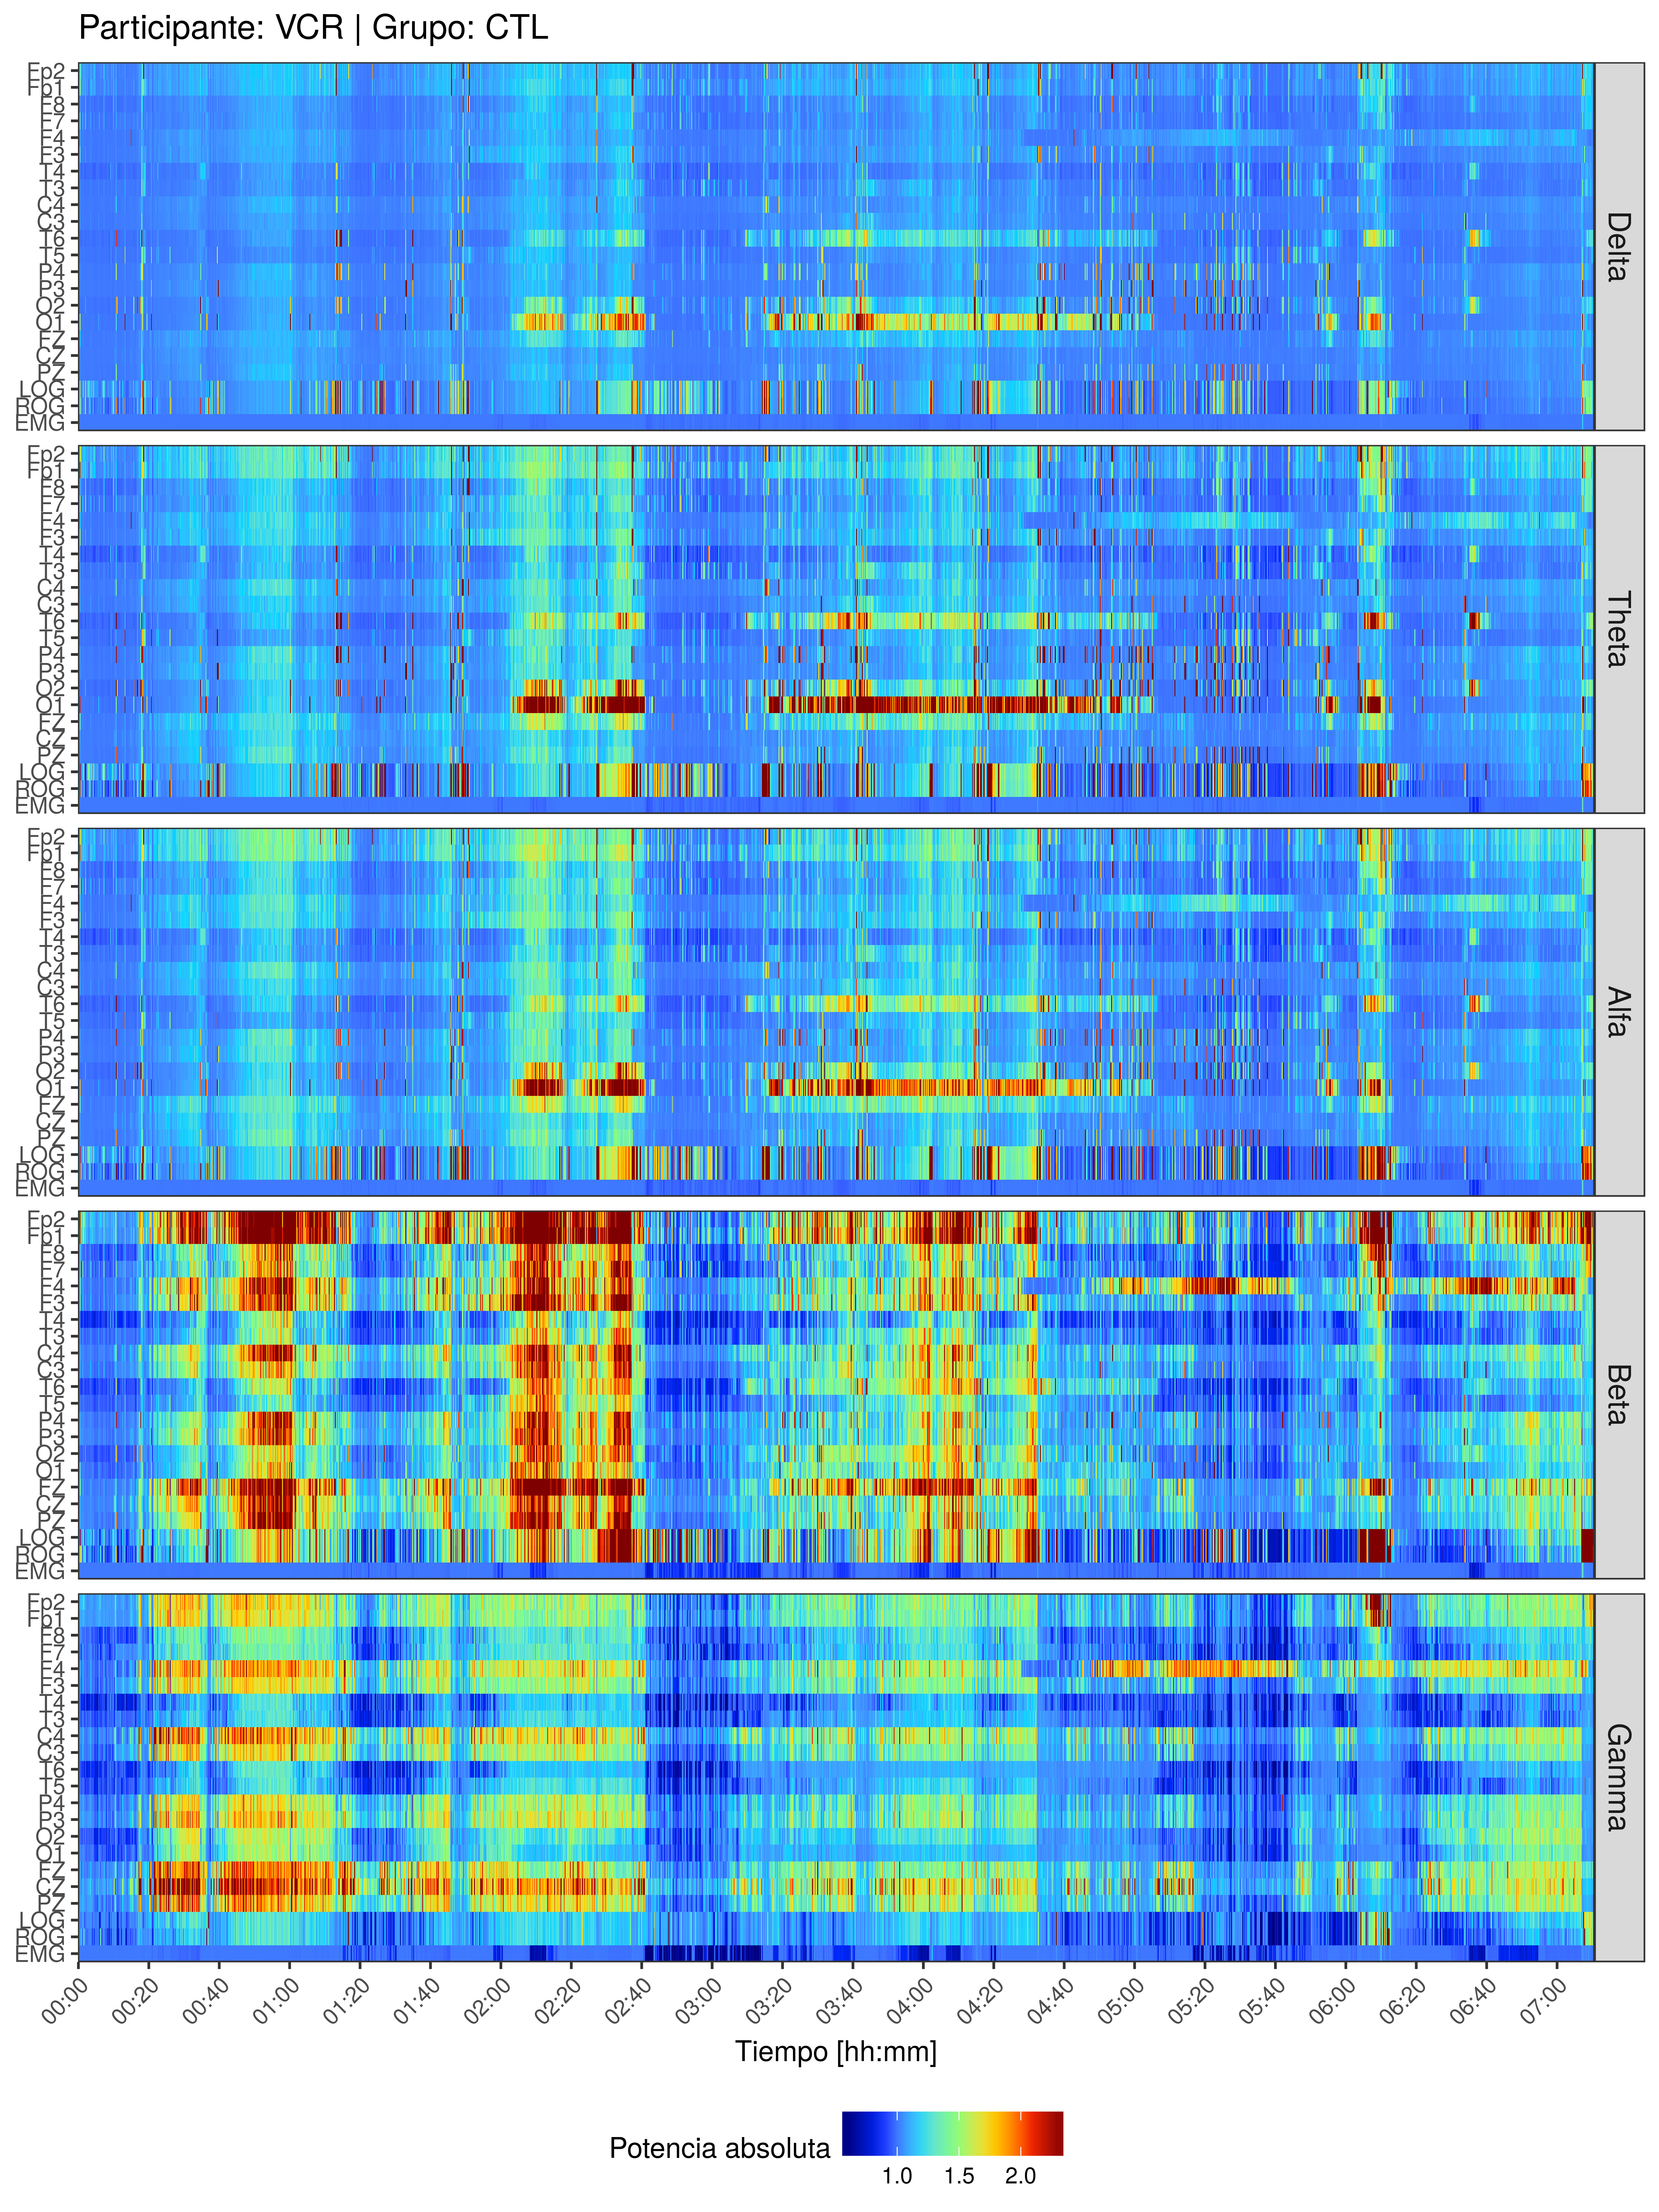
\includegraphics[width=\linewidth]
{./img_art_dfa/VCNNS1_espectral_total.png} 
\caption[Espectro de potencias de banda ancha]{Espectro de potencias de banda ancha (delta, theta
alfa, beta, gamma).}
\end{figure}

Usando los espectros de banda ancha se ha calculado el coeficiente de enlentecimiento \lento, 
definido en la 
expresión \ref{enlentecimiento}, con particular atención al sueño MOR. Esta cantidad
se ha reportado como un posible marcador de deterioro cognitivo leve en adultos mayores 
\cite{Brayet16}.

\begin{equation}
\text{R}_{\text{E}} = \frac{\text{potencia}_{\delta}+\text{potencia}_{\theta}}
{\text{potencia}_{\alpha}+\text{potencia}_{\beta}} =
\frac{\int_{\text 0.5 \hz}^{\text{7 \hz}}h(\omega) d\omega}
{\int_{\text 7 \hz}^{\text{30 \hz}}h(\omega) d\omega}
\label{enlentecimiento}
\end{equation}

El espectro de potencias se ha calculado usado el estimador adaptativo propuesto por
Barbour y Parker \cite{Barbour14}, el cual se encuentra implementado dentro del paquete
\texttt{psd} bajo la función \texttt{pspectrum}.
Se ha usado dicho estimador para garantizar heurísticamente que el espectro de potencias
calculado (1) es independiente del usado para determinar la estacionariedad y (2)
es compatible con la metodología \textit{usual}; como el algoritmo \texttt{psd} 
supone estacionariedad débil se espera que emule resultados 
obtenidos bajo tal supuesto.

Como se discute posteriormente, los bloques de épocas estacionarias están relacionados a bloques
cuyo espectro de potencia son distintos. Así mismo son diferentes los coeficientes \lento calculados
para dichos bloques.

%%%%%%%%%%%%%%%%%%%%%%%%%%%%%%%%%%%%%%%%%%%%%%%%%%%%%%%%%%%%%%%%%%%%%%%%%%%%%%%%%%%%%%%%%%%%%%%%%%%
%%%%%%%%%%%%%%%%%%%%%%%%%%%%%%%%%%%%%%%%%%%%%%%%%%%%%%%%%%%%%%%%%%%%%%%%%%%%%%%%%%%%%%%%%%%%%%%%%%%
%%%%%%%%%%%%%%%%%%%%%%%%%%%%%%%%%%%%%%%%%%%%%%%%%%%%%%%%%%%%%%%%%%%%%%%%%%%%%%%%%%%%%%%%%%%%%%%%%%%